\subsection{Perturbação de órbita fechada}\label{sec:2.10}
Até o presente momento, foram consideradas as trajetórias de um elétron em um campo guia pré-definido. Agora, deseja-se considerar a seguinte pergunta: suponha que toda a análise sobre a trajetória dos elétrons foi feita acerca de um campo guia pré-definido; como as trajetórias irão variar se existirem pequenos erros no campo com relação ao campo pré-definido? Considerando a aproximação linear realizada até aqui, o campo guia pré-definido -- ou nominal -- é especificado pelo seu valor na órbita ideal e sua derivada radial. Além disso, assume-se que o campo na órbita ideal é vertical em todo o anel. E se o campo magnético vertical na órbita ideal diferir do seu valor nominal, ou se existirem pequenas componentes horizontais de campo, as acelerações laterais serão diferentes das especificações necessárias para manter o elétron na órbita ideal. Os desvios do campo na órbita ideal serão chamam-se erros de campo, enquanto mudanças no campo que fazem com que as funções de focalização $K_x$ e $K_z$ tenham valores diferentes de seus valores nominais chamam-se erros de gradiente.

Quando existem erros de campo, a órbita ideal deixa de ser uma trajetória possível. Se os erros são pequenos, no entanto, irá existir uma outra órbita fechada a qual é uma trajetória possível a um elétron com energia nominal. Esta trajetória é chamada de órbita fechada. Esta trajetória irá executar as oscilações betatron relativas à órbita fechada. E a forma das oscilações betatron será determinada pelas novas funções de focalização. Isto é, mantendo $x$ como sendo a representação do desvio radial da órbita ideal, este pode ser descrito como
\begin{align}
	x = x_c + x_\beta\label{eq:2.83}
\end{align}
onde $x_c$ é o desvio da órbita fechada com relação à órbita ideal, e $x_\beta$ é a oscilação betatron com relação à órbita fechada.

Se os desvios da órbita fechada com relação à órbita ideal são pequenos, então as oscilações betatron são as mesmas, tanto com relação à órbita ideal quanto com relação à órbita fechada -- assumindo uma variação linear do campo. Desta forma, pode-se considerar separadamente a distorção da órbita fechada causada pelos erros de campo e os distúrbios nas oscilações betatron causados pelos erros de gradiente. Seguindo esta ideia, a equação \eqref{eq:2.83} pode ser interpretada como uma superposição da distorção da órbita fechada $x_c$ e a oscilação betatron $x_\beta$ calculada com relação à órbita ideal pelos métodos já estudados.

Analisando primeiramente os erros de campo. Suponha que os efeitos dos erros de campo existentes apenas em pequenos intervalos $\Delta s$ analisados a partir de $s=0$ comecem a ser considerados. Passando por $\Delta s$, o desvio $x$ não se altera, mas a inclinação $x'$ é alterada pela quantidade
\begin{align}
	\Delta x' = -\frac{ec\ \delta B}{E_0}\Delta s
\end{align}
onde $\delta B$ é o desvio do campo magnético com relação ao seu valor nominal.

\begin{proof}
	Fazendo um raciocínio bem informal, já foi visto que
	\begin{align*}
		d\theta = -\frac{ecB}{E}d\ell
	\end{align*}
	Considerando $d\ell$ pequeno, pode-se aproximar que $dx = d\ell$. Assim,
	\begin{align*}
		d\theta = -\frac{ecB}{E}ds
	\end{align*}
	Analisando apenas para uma pequena modificação no campo magnético, para um elétron com energia nominal:
	\begin{align*}
		d\theta = -\frac{ec\ \delta B}{E_0}ds
	\end{align*}
	Analisando para um intervalo $\Delta s$,
	\begin{align*}
		\Delta\theta = -\frac{ecB}{E}\Delta s
	\end{align*}
	Mas $\Delta \theta$ é a variação da inclinação $x'$, logo
	\begin{align*}
		\Delta x' = -\frac{ecB}{E}\Delta s
	\end{align*}
	Uma formulação mais rigorosa pode ser obtida analisando a força de Lorentz.
\end{proof}

Para o movimento vertical, pode-se obter uma equação da mesma forma se $\delta B$ for definido como o campo radial total na órbita ideal (com uma escolha adequada de sinal). Mantendo a definição da equação \eqref{eq:2.3}, tem-se que $-ec\ \delta B/E_0 = -\delta G$, considerando as coordenadas transversais $x$ e $z$. Para facilitar a análise, será considerada apenas uma coordenada $x$ genérica, lembrando que os resultados obtidos valem tanto para o movimento radial quanto para o vertical. Desta forma, pode-se reescrever a equação anterior como sendo
\begin{align}
	\Delta x' = -\delta G \Delta s\label{eq:2.84}
\end{align}

O erro de campo adiciona à relação $x'' = \Delta x'/ \Delta s$ o termo $-\delta G$; e é, portanto, equivalente a adicionar uma força direcional $\delta G(s)$ à equação de movimento. Pode-se obter a equação completa para $x_c$ adicionando esta nova força à equação diferencial de costume, equação \eqref{eq:2.31}:
\begin{align}
	x'' = -K(s)x - \delta G(s)\label{eq:2.85}
\end{align}
O desvio $x_c$ da órbita fechada é a solução desta equação singular.

Pode-se fazer uma estimativa do efeito de um erro de campo localizado em $s=0$ usando a forma harmônica aproximada do movimento betatron descrita na \autoref{sec:2.8}. Pense em um elétron viajando ao longo da órbita ideal -- de forma que a inclinação $x'$ seja nula. Quando este elétron chegar em $s=0$, sua inclinação será subitamente alterada para $\Delta x'$. Veja a \autoref{fig:fig21}. 

\begin{figure}[!htb]
	\centering
	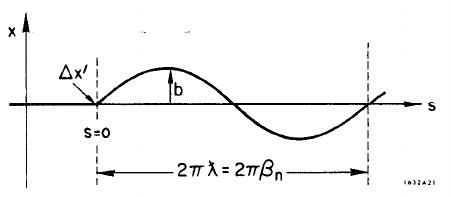
\includegraphics[width=0.7\linewidth]{./Figuras/fig21.jpeg}
	\caption{Efeito de um erro de campo localizado. Retirado de \cite{sands1970physics}.}
	\label{fig:fig21}
\end{figure}
Depois de $s=0$ não há erro de campo (para uma volta completa) então o elétron começa a oscilar em torno da órbita ideal com amplitude
\begin{align}
	b = \lambdabar \Delta x' = \beta_n \Delta x' = -\beta_n\ \delta G \Delta s\label{eq:2.86}
\end{align}
É esperado que o desvio da órbita fechada $x_c$ seja da mesma ordem de grandeza.

\begin{proof}
	Matematicamente, uma senoide com fase nula é descrita por
	\begin{align*}
		x(s) = b\ sen\left(\frac{2\pi s}{\lambda}\right)
	\end{align*}
	onde $b$ é a amplitude da oscilação e $\lambda$ é seu comprimento de onda. Desta forma,
	\begin{align*}
		x'(s) &= \frac{2\pi}{\lambda}b\ cos\left(\frac{2\pi s}{\lambda}\right)\\
		\therefore x'(0) & = \frac{2\pi}{\lambda}b\\
		\therefore b &= \frac{\lambda}{2\pi}x'(0)
	\end{align*}
	Já foi visto na \autoref{sec:2.8} que $\lambdabar = \lambda/2\pi$, então
	\begin{align*}
		b &= \lambdabar x'(0)
	\end{align*}
	Mas, considerando a análise que está sendo feita, $x'(0) = \Delta x'$. Logo,
	\begin{align*}
		b &= \lambdabar \Delta x'
	\end{align*}
	Também na \autoref{sec:2.8} mostrou-se que $\lambdabar = \beta_n$, então
	\begin{align*}
		b &= \beta_n \Delta x'\\
		  &= -\beta_n\ \delta G \Delta s
	\end{align*}
	c.q.d.
\end{proof}

Para fazer o cálculo de $x_c$ de forma apropriada, deve-se utilizar a oscilação pseudo-harmônica correta, e lembrar também que a órbita fechada é definida como a trajetória particular que fecha nela mesma após uma revolução. Em outras palavras, $x_c$ deve ser uma função singular em cada coordenada física $s$, ou seja, $x_c(s+L) = x_c(s)$. Em particular,
\begin{align}
	x_c(L) = x_c(0)\label{eq:2.87}
\end{align}
e, pela equação \eqref{eq:2.84},
\begin{align}
	x'_c(L) - \delta G \Delta s = x'_c(0)\label{eq:2.88}
\end{align}
Mas entre $s=0$ e $s=L$ não existem erros de campo, então $x_c$ é apenas uma oscilação livre entorno da órbita ideal. Veja a \autoref{fig:fig22}. Isto é, $x_c$ deve ser dado pela equação \eqref{eq:2.43}:
\begin{align}
	x_c(s) = a\sqrt{\beta(s)}cos(\varphi - \vartheta),\ s \neq 0,
\end{align}
com constantes arbitrárias $a$ e $\vartheta$ escolhidas de tal maneira que as equações \eqref{eq:2.87} e \eqref{eq:2.88} sejam satisfeitas.

\begin{figure}[!htb]
	\centering
	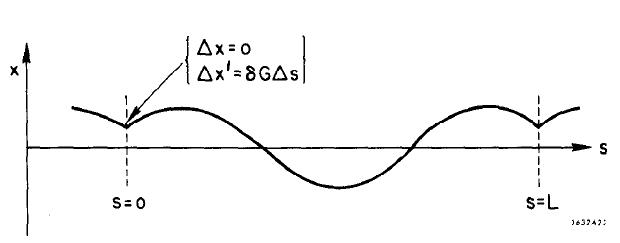
\includegraphics[width=0.7\linewidth]{./Figuras/fig22.jpeg}
	\caption{Órbita fechada para um erro de campo em $s=0$. Retirado de \cite{sands1970physics}.}
	\label{fig:fig22}
\end{figure}

Utilizando a equação \eqref{eq:2.52} para $x'_c(s)$ -- em todo o anel exceto em $s=0$ -- pode-se verificar que os valores apropriados para $a$ e $\vartheta$ são
\begin{align}
	a &= -\frac{\delta G\ \Delta s\ \sqrt{\beta(0)}}{2 sen(\pi \nu)}\\
	\vartheta &= \pi \nu
\end{align}

\begin{proof}
	Seja $x_c(L)$ dado pela equação \eqref{eq:2.89}:
	\begin{align*}
		x_c(L) = a\sqrt{\beta(L)}\ cos(\varphi(L)-\vartheta)
	\end{align*}
	Pela definição de $\varphi(s)$ e $\nu$,
	\begin{align*}
		x_c(L) = a\sqrt{\beta(L)}\ cos(2\pi\nu-\vartheta)
	\end{align*}
	Mas, a condição da equação \eqref{eq:2.87} deve ser satisfeita. Logo,
	\begin{align*}
		x_c(L) &= x_c(0)\\
		a\sqrt{\beta(L)}\ cos(2\pi\nu-\vartheta) &= a\sqrt{\beta(0)}\ cos(\varphi(0)-\vartheta)
	\end{align*}
	Novamente, pela definição de $\varphi(s)$,
	\begin{align*}
		a\sqrt{\beta(L)}\ cos(2\pi\nu-\vartheta) &= a\sqrt{\beta(0)}\ cos(-\vartheta)
	\end{align*}
	Pela periodicidade da função $\beta$,
	\begin{align*}
		a\sqrt{\beta(0)}\ cos(2\pi\nu-\vartheta) &= a\sqrt{\beta(0)}\ cos(-\vartheta)\\
		cos(2\pi\nu-\vartheta) &= cos(-\vartheta)
	\end{align*}
	Como cosseno é uma função par,
	\begin{align*}
		cos(2\pi\nu-\vartheta) &= cos(\vartheta)\\
		\therefore 2\pi\nu - \vartheta &= \vartheta\\
		\therefore \vartheta &= \pi\nu
	\end{align*}
	Agora, seja $x'_c(L)$ dado pela equação \eqref{eq:2.52}:
	\begin{align*}
		x'_c(L) &= -\frac{a}{\beta(L)}\ sen(\varphi(L)-\vartheta) + \frac{\beta'(L)}{2\beta(L)}x_c(L)\\
				&= -\frac{a}{\beta(L)}\ sen(2\pi\nu-\pi\nu) + \frac{\beta'(L)}{2\beta(L)}x_c(L)\\
				&= -\frac{a}{\beta(L)}\ sen(\pi\nu) + \frac{\beta'(L)}{2\beta(L)}x_c(L)
	\end{align*}
	A condição da equação \eqref{eq:2.88} impõe que
	\begin{align*}
		x'_c(L) - \delta G\ \Delta s &= x'_c(0)\\
		-\frac{a}{\beta(L)}\ sen(\pi\nu) + \frac{\beta'(L)}{2\beta(L)}x_c(L) - \delta G\ \Delta s &= -\frac{a}{\beta(0)}\ sen(\varphi(0)-\pi\nu) + \frac{\beta'(0)}{2\beta(0)}x_c(0)\\
		-\frac{a}{\beta(L)}\ sen(\pi\nu) + \frac{\beta'(L)}{2\beta(L)}x_c(L) - \delta G\ \Delta s &= -\frac{a}{\beta(0)}\ sen(0-\pi\nu) + \frac{\beta'(0)}{2\beta(0)}x_c(0)\\
		-\frac{a}{\beta(L)}\ sen(\pi\nu) + \frac{\beta'(L)}{2\beta(L)}x_c(L) - \delta G\ \Delta s &= -\frac{a}{\beta(0)}\ sen(-\pi\nu) + \frac{\beta'(0)}{2\beta(0)}x_c(0)
	\end{align*}
	Pela periodicidade da função $\beta(s)$ e a restrição imposta pela equação \eqref{eq:2.87},
	\begin{align*}
		-\frac{a}{\beta(0)}\ sen(\pi\nu) + \frac{\beta'(0)}{2\beta(0)}x_c(0) - \delta G\ \Delta s &= -\frac{a}{\beta(0)}\ sen(-\pi\nu) + \frac{\beta'(0)}{2\beta(0)}x_c(0)\\
		\therefore -\frac{a}{\beta(0)}\ sen(\pi\nu) - \delta G\ \Delta s &= -\frac{a}{\beta(0)}\ sen(-\pi\nu)
	\end{align*}
	Como seno é uma função ímpar,
	\begin{align*}
		-\frac{a}{\beta(0)}\ sen(\pi\nu) - \delta G\ \Delta s &= \frac{a}{\beta(0)}\ sen(\pi\nu)\\
		\therefore \frac{a}{\beta(0)}\ 2sen(\pi\nu) &= -\delta G\ \Delta s\\
		\therefore a = -\frac{\delta G\ \Delta s\ \sqrt{\beta(0)}}{2 sen(\pi \nu)}
	\end{align*}
	c.q.d.
\end{proof}

O desvio da órbita fechada é, portanto,
\begin{align}
	x_c(s) = -\frac{\delta G\ \Delta s\ \sqrt{\beta(0)}}{2 sen(\pi \nu)}\ \sqrt{\beta(s)}\ cos(\varphi(s)-\pi\nu)\label{eq:2.92}
\end{align}

A forma do invariante $a$ da amplitude mostra duas características interessantes da órbita fechada. Primeiramente, note que o desvio da órbita fechada é em todo o anel proporcional à "força" $\ \delta G \Delta s$ do erro de campo, e à raiz de $\beta(0)$, a magnitude da função betatron no local da perturbação. Agora entende-se porque $\beta(s)$ -- ou mais precisamente $\zeta(s) = \sqrt{\beta(s)}$ -- é uma medida da "sensibilidade" à distúrbios.

Segundo, note que o denominador de $a$ vai para zero, e $x_c$ se torna, portanto, muito grande sempre que a sintonia $\nu$ se aproxima de um inteiro. É este comportamento o qual foi referido anteriormente como "ressonância inteira", a qual deve ser evitada escolhendo o ponto de operação $(\nu_x,\nu_z)$ longe de números inteiros.

Note que o desvio da órbita fechada no local do erro de campo tem uma forma particularmente simples. Basta apenas analisar a equação \eqref{eq:2.92} considerando $s=0$, ou generalizar para um erro de campo localizado em uma coordenada arbitrária $s_1$, obtendo
\begin{align}
	x_c(s_1) = -\delta G\ \Delta s \frac{\beta(s_1)}{2 tg(\pi\nu)}
\end{align}
Agora o desvio é proporcional à primeira potência de $\beta$, mas a dependência da ressonância de $\nu$ ainda é evidente no termo da tangente. Note também que, exceto pelo denominador ressonante, o resultado confere com a estimativa dada pela equação \eqref{eq:2.86}.

A equação \eqref{eq:2.92} também pode ser generalizada para uma órbita fechada com erros de campo que seguem uma distribuição arbitrária ao longo do anel. Em cada coordenada $s$, os desvios da órbita fechada causados por erros em todas as outras coordenadas irão se somar. Para um erro em $\bar{s}$, deve-se substituir $s=0$ por $\bar{s}$ na equação \eqref{eq:2.92} -- e, ao mesmo tempo, substituir $\varphi(s)$ por $|\varphi(s) - \varphi\bar{s}|$. Assim, somando sobre todos os $\Delta \bar{s}$, tem-se 
\begin{align}
	x_c(s) = -\frac{\sqrt{\beta(s)}}{2sen(\pi\nu)}\int\limits_{0}^{L}\delta G(\bar{s})\sqrt{\beta(\bar{s})}cos(|\varphi(s)-\varphi(\bar{s})|-\pi\nu)d\bar{s}\label{eq:2.94}
\end{align}
Se o desvio de campo $\delta G(s)$ é conhecido, esta equação dará a forma da órbita fechada (considerando os valores nominais de $\beta(s)$ e $\nu$).

Se os desvios de campo são verdadeiros "erros" com uma distribuição estatística desconhecida, uma análise estatística mais complexa deve ser feita para chegar na estimativa estatística de $x_c$.

Como foi dito anteriormente, o desvio total da órbita ideal é dado pela soma de $x_c$ e a oscilação betatron. Na próxima análise, $x_c$ será ignorado -- lembrando sempre que este precisa ser adicionado quando pretende-se analisar o desvio total da trajetória com relação à órbita ideal.